\chapter{Experimentation and results}
\label{Chapter4}

After having explained the necessary theoretical background and presented the proposals
of this work, it is time that we put them into action to see how they perform. First, we are going
to test our proposals on some toy datasets in order to better understand them. After that, we are going
to try the proposed invariants as well as the multiclass extension with ECOC on real data to see how
well they perform when comparing them to the original invariants proposed in \cite{Vapnik2019}.

\section{Experimenting with toy problems}


\begin{figure}
    \centering
    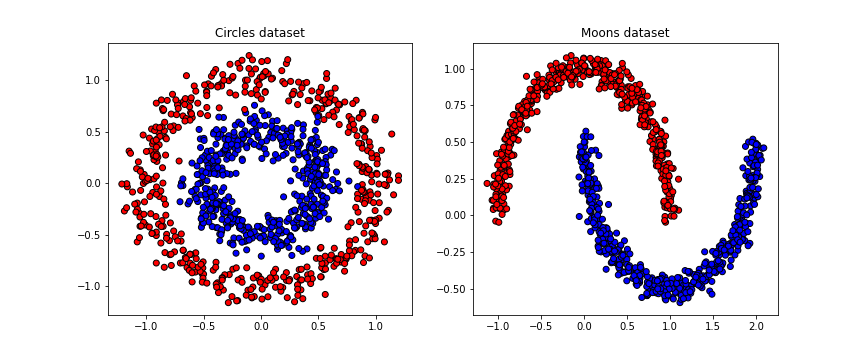
\includegraphics[width=\textwidth]{thesis/Figures/toy_datasets.png}
    \caption{Toy datasets used in the experimentation.}
    \label{fig:toy_datasets}
\end{figure}

\begin{figure}
    \centering
    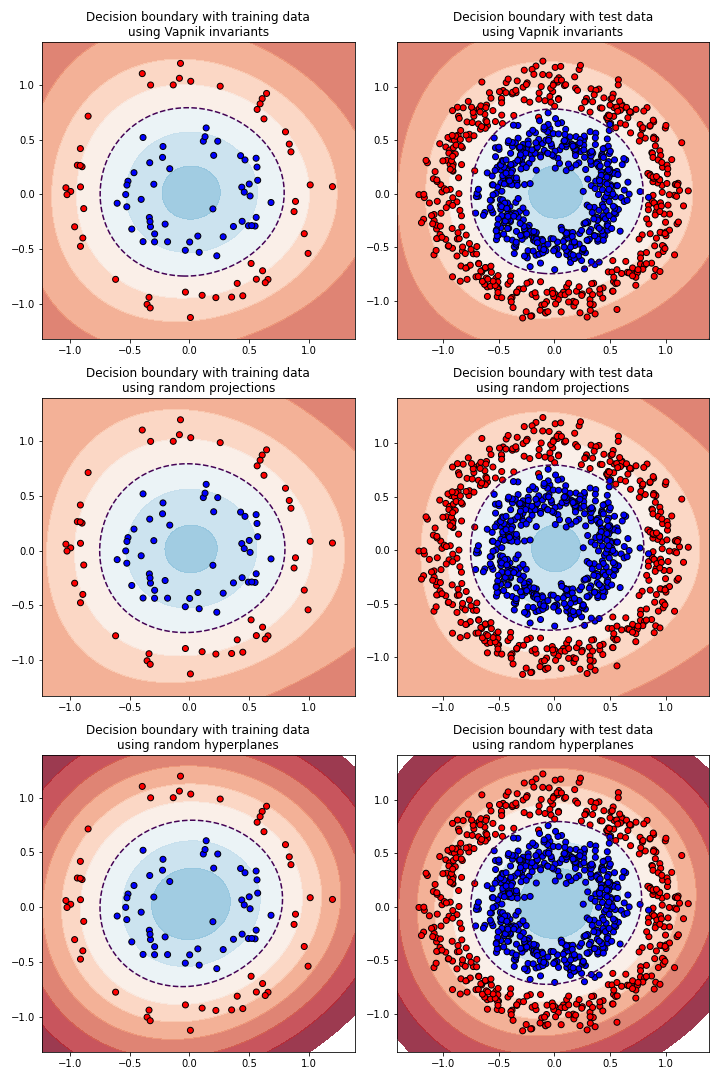
\includegraphics[width=\textwidth]{thesis/Figures/circles_decision_boundaries.png}
    \caption{Caption}
    \label{fig:circles_decision_boundary}
\end{figure}

\begin{figure}
    \centering
    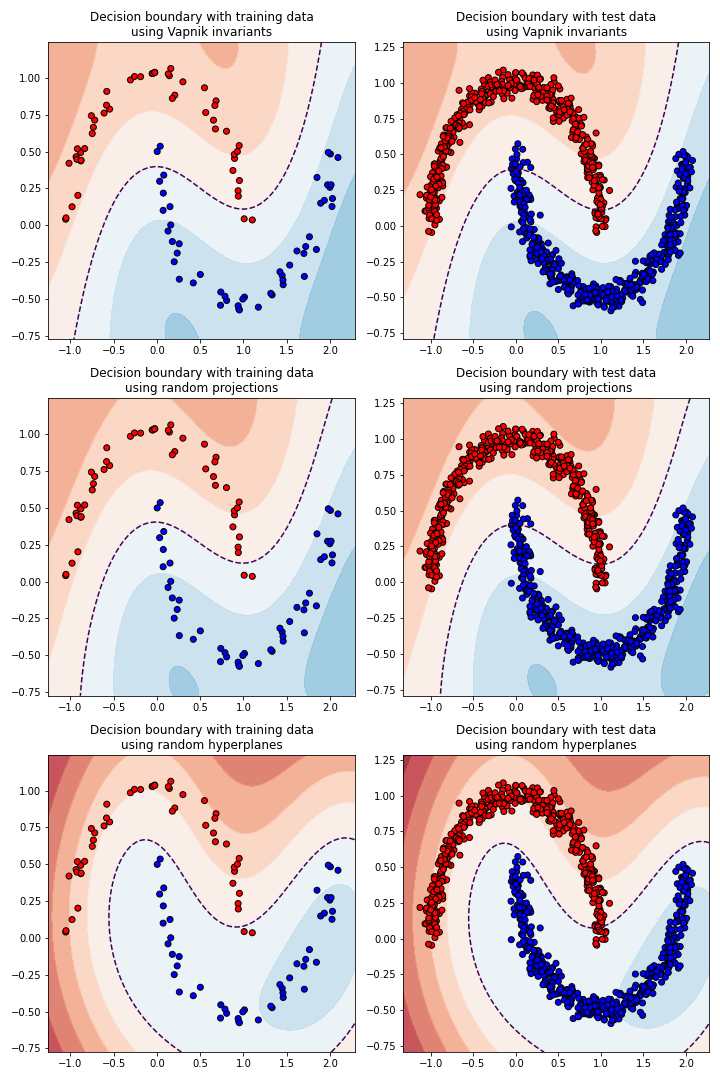
\includegraphics[width=\textwidth]{thesis/Figures/moons_decision_boundaries.png}
    \caption{Caption}
    \label{fig:moons_decision_boundary}
\end{figure}

\begin{figure}
    \centering
    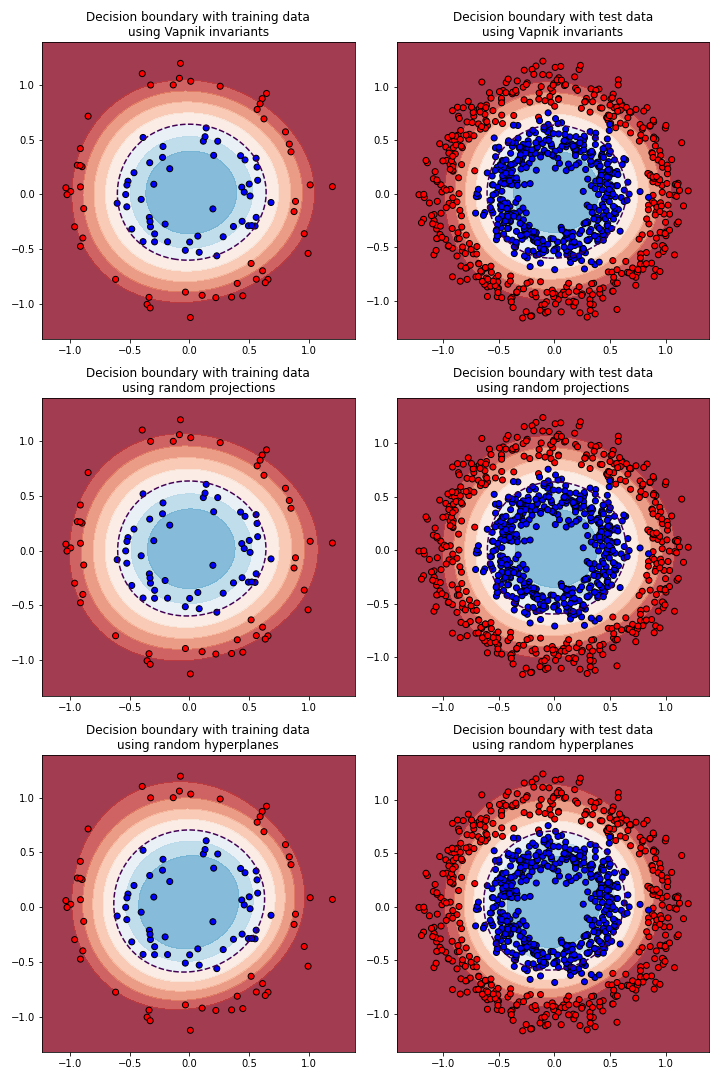
\includegraphics[width=\textwidth]{thesis/Figures/circles_decision_boundaries_ecoc.png}
    \caption{Caption}
    \label{fig:circles_decision_boundary_ecoc}
\end{figure}

\begin{figure}
    \centering
    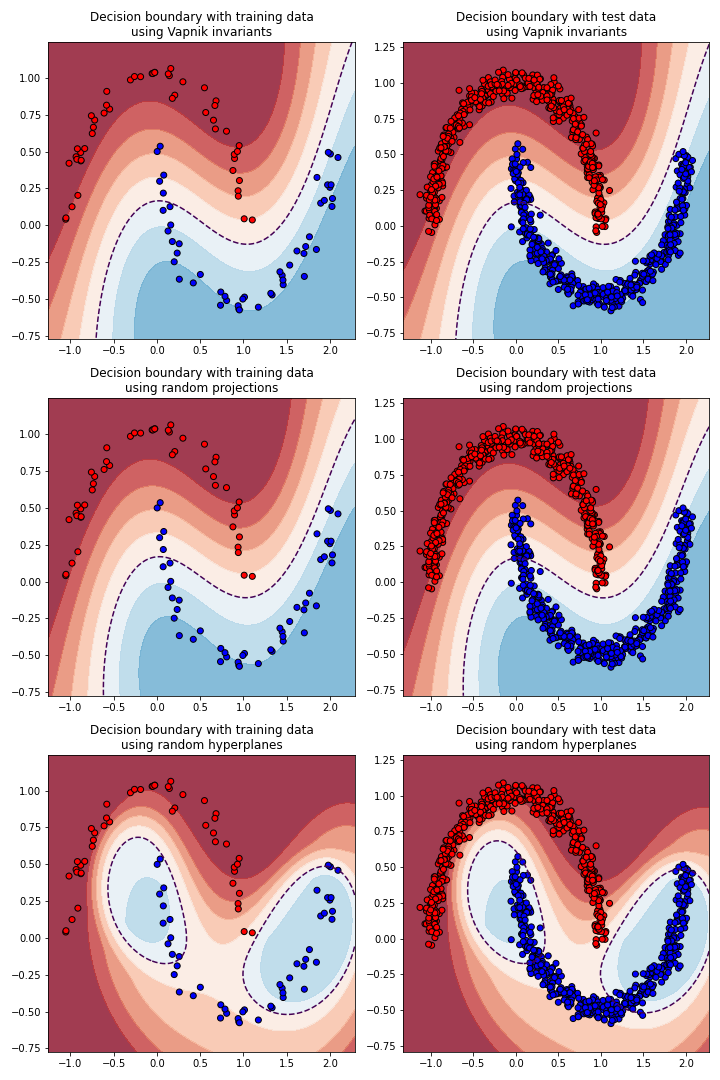
\includegraphics[width=\textwidth]{thesis/Figures/moons_decision_boundaries_ecoc.png}
    \caption{Caption}
    \label{fig:moons_decision_boundary_ecoc}
\end{figure}

\begin{figure}
    \centering
    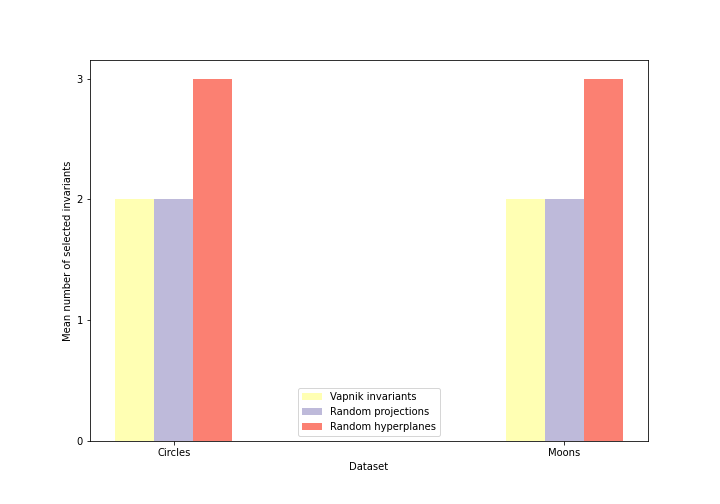
\includegraphics[width=0.8\textwidth]{thesis/Figures/num_selected_invariants.png}
    \caption{Caption}
    \label{fig:toys_small_num_selected_invariants}
\end{figure}

\begin{figure}
    \centering
    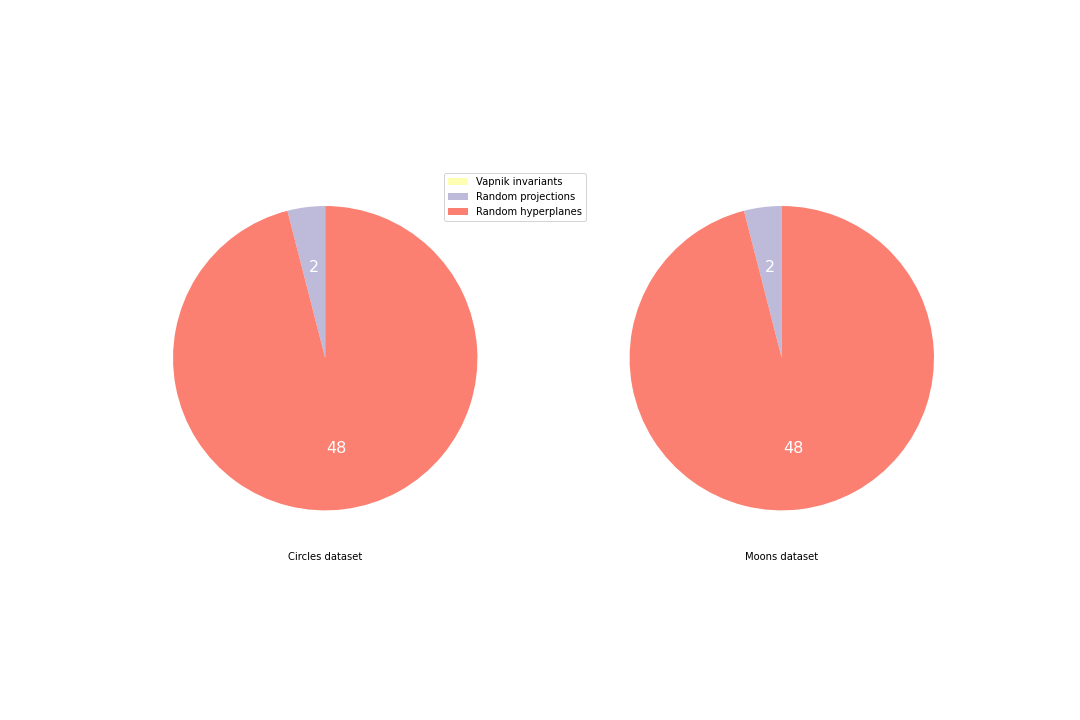
\includegraphics[width=\textwidth]{thesis/Figures/mean_num_selected.png}
    \caption{Caption}
    \label{fig:toys_mean_num_selected}
\end{figure}



\section{Experimentation on real data}
\subsection{Experimental settings}
{\bf Data:} Datos y tabla resumen de los datasets\\
{\bf Baselines:} Que métodos vas a comparar.
SVM sin invariantes
SVM con invariantes Vapnik
SVM con invariantes Vladis

Todos con el mismo sistema de selección.
\\
{\bf Methodology and performance metrics:} XValidation? cuanto, como mides los resultados?

Accuracy promedio i desviación estandar.
\\
{\bf Experimental and parameter setting:}
Haces parameter tunning?

Que experimentos propones?

1- Experimento base: Todos los datos con los modelos a comparar\\
2- Experimento con reduccion de datos.

\begin{table}[H]
\centering
\begin{tabular}{lrrr}
\textbf{Problem} & \textbf{Num. examples} & \textbf{Attributes} & \textbf{Classes} \\ \hline
Balance scale    & 625                    & 4                   & 3                \\
Ecoli            & 336                    & 8                   & 8                \\
Glass            & 214                    & 9                   & 7(6)\tablefootnote{According to the dataset's documentation, there are 7 classes. However, there is one that does not have any elements. Therefore, the actual number of classes for this problem is 6.}                \\
Iris             & 150                    & 4                   & 3                \\
Yeast            & 1484                   & 8                   & 10              
\end{tabular}
\caption{Caption}
\label{tab:problems_description}
\end{table}


\subsection{Results}

% Please add the following required packages to your document preamble:
% \usepackage{graphicx}
\begin{table}[h]
\centering
\resizebox{\textwidth}{!} &
  10\% &
  \multicolumn{1}{c|}{100\%} &
  10\% &
  \multicolumn{1}{c|}{100\%} &
  10\% &
  \multicolumn{1}{c|}{100\%} &
  10\% \\ \hline
\multicolumn{1}{|c|}{Balance scale} &
  \multicolumn{1}{c|}{$91.47 \pm 0.38\%$} &
  $88.80 \pm 1.73\%$ &
  \multicolumn{1}{c|}{$91.47 \pm 0.38\%$} &
  $87.73 \pm 2.10\%$ &
  \multicolumn{1}{c|}{$91.73 \pm 0.38\%$} &
  $83.73 \pm 7.17\%$ &
  \multicolumn{1}{c|}{$90.13 \pm 1.51\%$} &
  $76.00 \pm 12.77\%$ \\ \hline
\multicolumn{1}{|c|}{Ecoli} &
  \multicolumn{1}{c|}{$85.29 \pm 2.08\%$} &
  $71.57 \pm 1.39\%$ &
  \multicolumn{1}{c|}{$85.29 \pm 1.20\%$} &
  $72.55 \pm 4.22\%$ &
  \multicolumn{1}{c|}{$84.15 \pm 2.05\%$} &
  $67.32 \pm 4.03\%$ &
  \multicolumn{1}{c|}{$75.98 \pm 6.28\%$} &
  $63.89 \pm 9.61\%$ \\ \hline
\multicolumn{1}{|c|}{Glass} &
  \multicolumn{1}{c|}{$72.87 \pm 7.91\%$} &
  $56.59 \pm 4.78\%$ &
  \multicolumn{1}{c|}{$72.87 \pm 7.91\%$} &
  $45.74 \pm 6.67\%$ &
  \multicolumn{1}{c|}{$72.09 \pm 7.44\%$} &
  $52.45 \pm 7.03\%$ &
  \multicolumn{1}{c|}{$71.06 \pm 7.60\%$} &
  $45.48 \pm 9.50\%$ \\ \hline
\multicolumn{1}{|c|}{Iris} &
  \multicolumn{1}{c|}{$96.67 \pm 0.00\%$} &
  $93.33 \pm 2.72\%$ &
  \multicolumn{1}{c|}{$95.56 \pm 1.57\%$} &
  $90.00 \pm 4.71\%$ &
  \multicolumn{1}{c|}{$95.19 \pm 1.66\%$} &
  $77.78 \pm 22.93\%$ &
  \multicolumn{1}{c|}{$88.52 \pm 11.56\%$} &
  $84.81 \pm 9.04\%$ \\ \hline
\multicolumn{1}{|c|}{Yeast} &
  \multicolumn{1}{c|}{$53.76 \pm 1.04\%$} &
  $47.92 \pm 2.08\%$ &
  \multicolumn{1}{c|}{$53.87 \pm 1.20\%$} &
  $47.92 \pm 2.14\%$ &
  \multicolumn{1}{c|}{$52.53 \pm 5.44\%$} &
  $45.68 \pm 4.60\%$ &
  \multicolumn{1}{c|}{$50.39 \pm 5.33\%$} &
  $37.82 \pm 7.92\%$ \\ \hline
\end{tabular}%
}
\caption{Caption}
\label{tab:results_accuracies_errors}
\end{table}

\begin{figure}
    \centering
    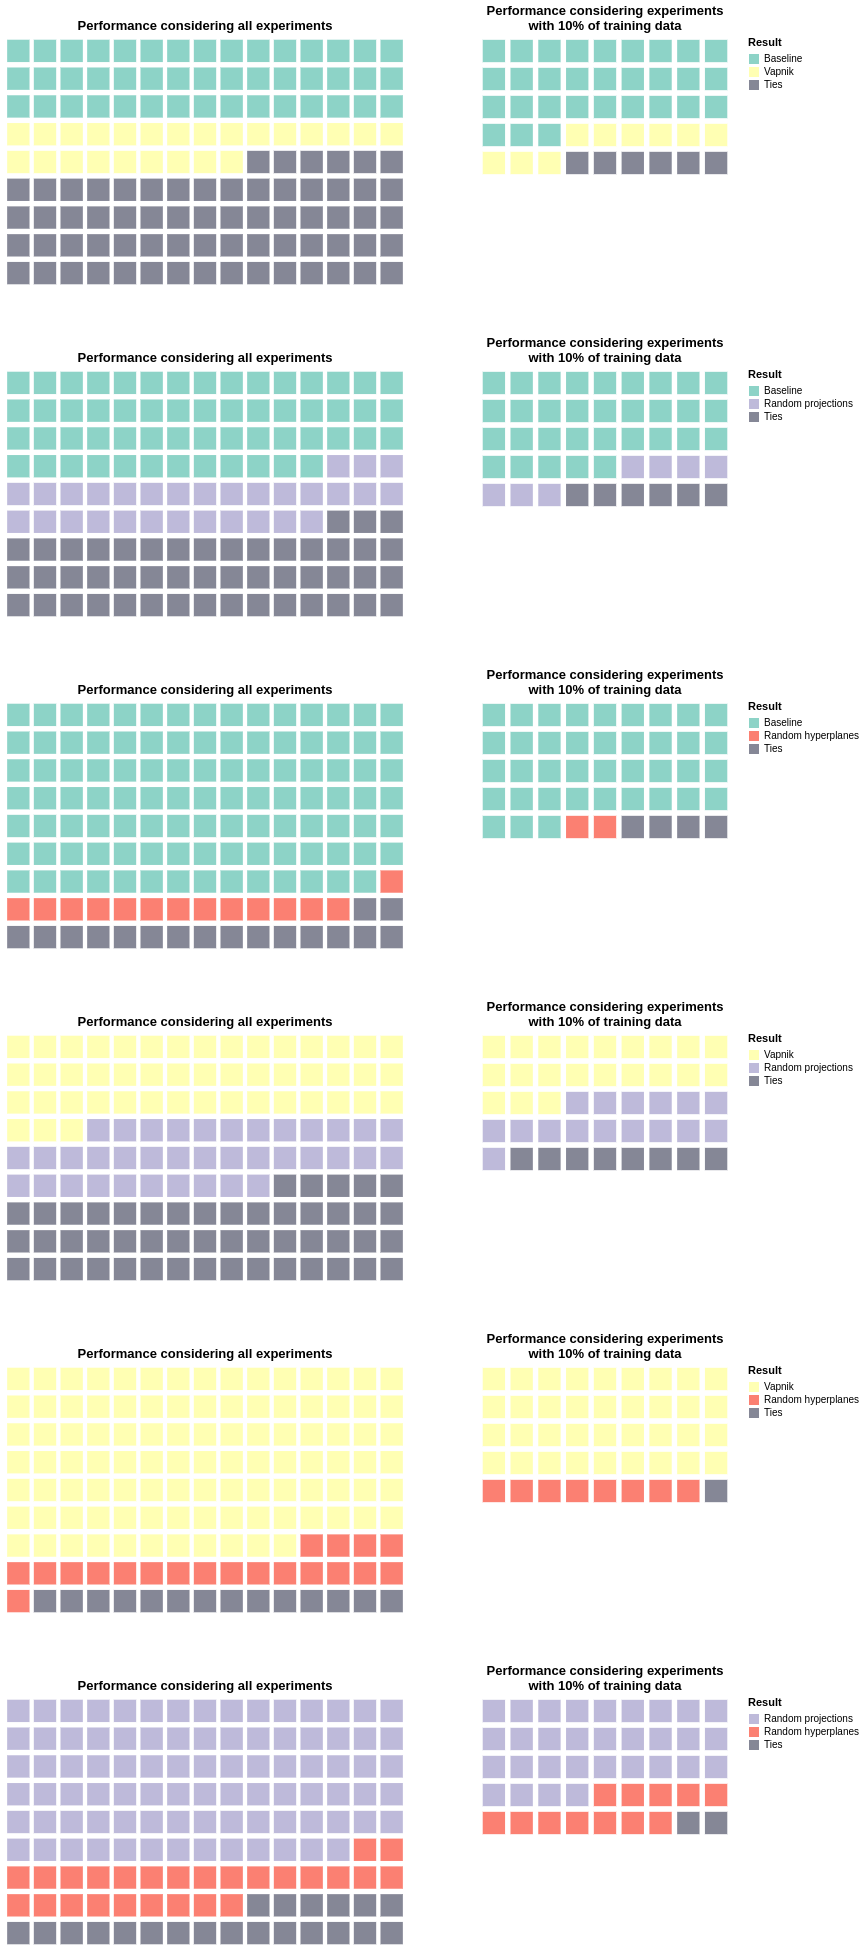
\includegraphics[width=0.7\textwidth]{thesis/Figures/invariants_performance.png}
    \caption{Caption}
    \label{fig:invariants_performance}
\end{figure}